\documentclass{bmvc2k}

%% Enter your paper number here for the review copyu
\bmvcreviewcopy{123}

\title{Single View Correspondence Matching for Non-Coplanar Circles Using Euclidean Invariants}

% Enter the paper's authors in order
% \addauthor{Name}{email/homepage}{INSTITUTION_CODE}
\addauthor{Susan Student}{http://www.vision.inst.ac.uk/~ss}{1}
\addauthor{Petra Prof}{http://www.vision.inst.ac.uk/~pp}{1}
\addauthor{Colin Collaborator}{colin@collaborators.com}{2}

% Enter the institutions
% \addinstitution{Name\\Address}
\addinstitution{
 The Vision Institute\\
 University of Borsetshire\\
 Wimbleham, UK
}
\addinstitution{
 Collaborators, Inc.\\
 123 Park Avenue,\\
 New York, USA
}
\usepackage[]{algorithm2e}

% added by Yuji
%%%%%%%% FROM HERE
\usepackage{color}
\newcommand{\parmessage}[1]{\textcolor{cyan}{[Paragraph: #1]}}
\newcommand{\comments}[1]{\textcolor{magenta}{[Comments: #1]}}
\newcommand{\yuji}[1]{\textcolor{magenta}{[Yuji: #1]}}
\newcommand{\revise}[2]{\textcolor{red}{\sout{#1}} \textcolor{blue}{#2}}  %Before (magenta) and after (blue)
%\newcommand{\revise}[2]{\textcolor{green}{#1}}  %Modifications appear in green
%\newcommand{\revise}[2]{#1} % Just the modified result
%\newcommand{\revise}[2]{#2} % Before the modification
\usepackage{ulem}

\newcommand{\fref}[1]{Fig\bmvaOneDot~\ref{#1}}
\newcommand{\Fref}[1]{Figure~\ref{#1}}
\newcommand{\eref}[1]{Eq\bmvaOneDot~\ref{#1}}
\newcommand{\Eref}[1]{Equation~\ref{#1}}
\newcommand{\sref}[1]{Sec\bmvaOneDot~\ref{#1}}
\newcommand{\Sref}[1]{Section~\ref{#1}}
%%%%%%%% UNTIL HERE

\runninghead{Student, Prof, Collaborator}{BMVC Author Guidelines}

% Any macro definitions you would like to include
% These are not defined in the style file, because they don't begin
% with \bmva, so they might conflict with the user's own macros.
% The \bmvaOneDot macro adds a full stop unless there is one in the
% text already.
\def\eg{\emph{e.g}\bmvaOneDot}
\def\Eg{\emph{E.g}\bmvaOneDot}
\def\etal{\emph{et al}\bmvaOneDot}

%------------------------------------------------------------------------- 
% Document starts here
\begin{document}

\maketitle

\begin{abstract}
In this work we introduce a method to determine 2D-3D correspondence for non-coplanar circles using a single image, given that the 3D information is known. 
%the orientation of circle plane is known. 
The core idea of our method is to compute 3D information from 2D features, thereby transforming a 2D-3D problem to a 3D-3D problem. 
Earlier researchers suggested that a pair of non-coplanar circles preserves Euclidean invariants under perspective projection.
These invariants can be extracted from their image projections, but with a two fold ambiguity. 
In this paper, we propose \textit{Conic pair descriptor} based on the Euclidean invariants.
The proposed descriptor computes unique Euclidean invariants from known 3D model and Euclidean invariants with two fold ambiguity from its image projections.
The proposed matching approach follows three steps to obtain correspondences between the circular features against the ambiguity.
In this paper, we have included a detailed account of factors affecting the computation of invariants from conic projections. 
%\yuji{Our method can be used for any 3D object having identical circular features on different planes.}{}
We have conducted experiments on real and synthetic models, in order to evaluate the proposed method. 
The experiment with synthetic images focuses on showing the impact of the size and plane orientation of the circles on the success of descriptor matching. 
%The experiments with synthetic images provide understanding of variation in matching success with respect to the orientation and size of the circles. 
We prepared 3D models with artificial circular features and obtained the ground truth 3D data with a Photogrammetric measurement system. 
The results of the correspondence matching algorithm are evaluated against the ground truth. 
We also show that our method is robust against false positives and capable of supporting real-time applications.   

%\yuji{We endorse our method for model based tracking applications in the industrial domain, where natural or artificial circular features readily exist on the model.}{}
%which is supported our claim and show compatibility with proposed industrial applications. 

\end{abstract}

%------------------------------------------------------------------------- 
\section{Introduction}
\label{sec:intro}
%goal : 
%Explain the problem in question, the motivation for the work and the proposed application in mind. The assumptions made in our work. We have the camera calibrated and we use 3D points and their normal positions for the descriptor measurement. 
%No much work done in this direction. The invariants proposed are never used for a application so we provide use and discuss stability of the algorithm. Comment on why circles and the paper we build up to. 
%The work of Forsyth as the base of our work, the concepts given in the paper. Our contribution is matching strategy using such invariants. Demonstrating an application and evaluation of the method. 

Correspondence matching is one of the key problems in computer vision.
Pose estimation and object recognition applications require accurate knowledge of correspondence relation \yuji{($ m_i \leftrightarrow M_i $)}{$ m_i \leftrightarrow M_i $} between 3D model features \yuji{($ M_i $)}{$ M_i $} and 2D image features \yuji{($ m_i $)}{$ m_i $}. 
In case of monocular systems the \yuji{$ m_i \leftrightarrow M_i $}{2D-3D correspondence} problem becomes more challenging as the depth information is lost.
Various Computer Vision and Augmented Reality applications demand correspondence matching from a single view.
Popular approach to achieve this is to compute projective invariant from features \yuji{like}{such as} points, lines and conics \cite{hartley_multiple_2003}.
Such features are \yuji{selected}{preferred} because they are easier to detect from the images. 
Invariants are extensively studied topic in vision community, Forsyth \etal \cite{forsyth_91} and Gros \cite{gros_projective_1992} covered a detailed study on \yuji{projective invariant descriptors}{projective invariants} and their stability under projective transformation. 
In this paper we will focus on a specific class of features, that is \textit{circles}. 
Circles are one of the most primitive features\yuji{,}{.}
In case of industrial scenario circles are widely present on the model as natural features or circular fiducial are used for Photogrammetric measurements \cite{luhmann_close_2006} (\yuji{}{see} \fref{fig:introProblem}).
In such cases it is favourable to build tracking approach depending on such features. 
A single view correspondence matching problem with coplanar circles and ellipses is widely studied \cite{lepetit_monocular_2005}\yuji{,}{.}
However matching problem with non-coplanar circles has not been addressed. 
\Fref{fig:introProblem} shows a basic example of the problem, where multiple identical circular features exist on different planes of a 3D model.
In this case features existing on the model is an advantage, but coplanar invariants can not be used for correspondence matching.
In out work we focus on solving this problem of single view matching of multiple non coplanar conics. 

%In learning based model tracking methods initial frames of the camera are used to learn model and compute unique descriptors from dense or sparse set of natural model features \cite{chekhlov_ninja_2007} \cite{hinterstoisser_n3m:_2007} \cite{lowe_object_1999}. Other methods involve using a selective set features (edges, contours, etc.) to compute invariants from a single image \cite{lepetit_monocular_2005}. 

\begin{figure}
\centering
\begin{tabular}{cc}
%\bmvaHangBox{\fbox{\includegraphics[width=5cm,height =3cm]{images/Problem.png}} }&
%\bmvaHangBox{\fbox{\includegraphics[width=5cm,height = 3cm]{images/carModels.png}} } \\ %keepaspectratio=true
\bmvaHangBox{\fbox{\includegraphics[width=0.57\hsize]{images/Problem.png}} }&
\bmvaHangBox{\fbox{\includegraphics[width=0.3\hsize]{images/carModels.png}} } \\ %keepaspectratio=true
(a)&(b)
\end{tabular}
\caption{ Matching problem for non-coplanar circles ;
(a) A primitive example explaining the problem when image features have same properties and correspondence relation with model is ambiguous (b) A realistic model prepared with circular fiducials used for Photogrammetric measurements in Industry
\comments{(1) better to add caption to (a) and (b) so that the readers can easily get what they are. (2) better to save all figures as vector image files as .eps and .pdf so that the figures can keep its visual even when they are zoomed up.}
}
\label{fig:introProblem}
\end{figure}

%In single images projective transformation of features make it difficult to compute invariant features. 
3D objects retain Euclidean invariants rather than projective invariants \cite{forsyth_91}. 
In case of 3D objects Euclidean invariants are difficult to extract from images due to perspective mapping. 
Circles have a special property to retain depth information under projective transformation.
A world circle always produces an elliptical curve on the image plane.
If size of circle is known orientation of circle plane can be defined in 3D (camera coordinates) with a two fold ambiguity \cite{forsyth_91} \cite{safaee-rad_three-dimensional_1992}. 
Further, Forsyth \etal \cite{forsyth_91} proposed that up to three projective invariant can be computed from a non-coplanar pair of circles.
They explain that angle between circle planes (angle between surface normals) and distance between centre of the circles are invariant quantities.
The concept was proposed in early 90s, however these invariants have remained unexplored. 
We propose using these invariants to solve correspondence problem when multiple 3D circular features exist on a model. 
In this approach we bring problem from 2D to 3D by computing 3D invariants from image features, then solve 3D-3D matching problem with model.
We introduce $ Conic Pair Descriptor $, which encapsulate invariants computed from elliptical image features to solve the conic ambiguity and provide accurate matching with 3D features. 
The proposed method is first attempt to use these invariants, therefore we also carried out simulations to show stability of invariants against change of perspective.  

%We demonstrate  practical scenario where such method can be used effectively.
Our contribution is a new method to accurately identify image correspondences when multiple identical 3D circular features exist in the scene. We assume that calibration of camera is known and 3D information of features is available. 
Often in Industry based model tracking applications 3D-CAD data is known. Our matching method is suitable for tracking any 3D objects having known circles on different planes. In close range photogrammetry multiple circular markers (Figure. \ref{fig:introProblem}) are placed on 3D models for surface measurements \cite{luhmann_close_2006}. 
These measurements include computation of surface normal and 3D position of each marker. 
This process involves taking multiple images of the model with additional presence of encoded markers in the scene to solve correspondence. 
Once 3D measurements are done our method can be extremely useful to support tracking application without using coded patterns. Similarly various industrial parts having natural circles can be identified and tracked with this method. 
We prepared two car models with circular markers for evaluating our matching method. The proposed method can find corresponding circular marker from a single image, with high accuracy. We also show that our method is stable against false positives detected from the scene. Our method is fast enough to support real-time tracking applications. 


%-> Figure explaining the issue 
%\begin{figure}
%\begin{tabular}{ccc}
%\bmvaHangBox{\fbox{\parbox{2.7cm}{~\\[2.8mm]
%\rule{0pt}{1ex}\hspace{2.24mm}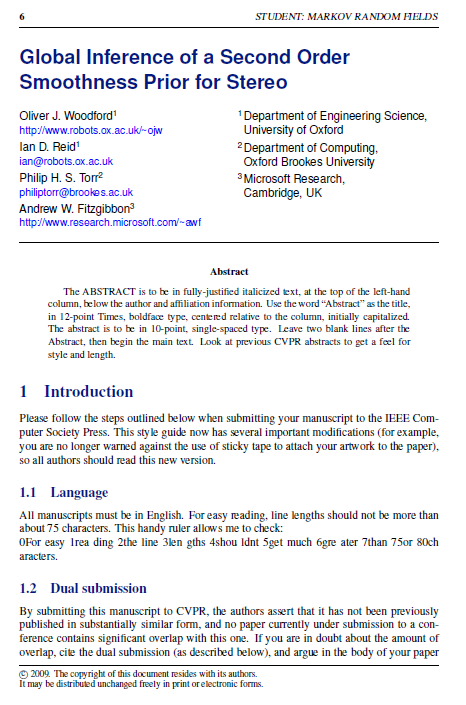
\includegraphics[width=2.33cm]{images/eg1_largeprint.png}\\[-0.1pt]}}}&
%\bmvaHangBox{\fbox{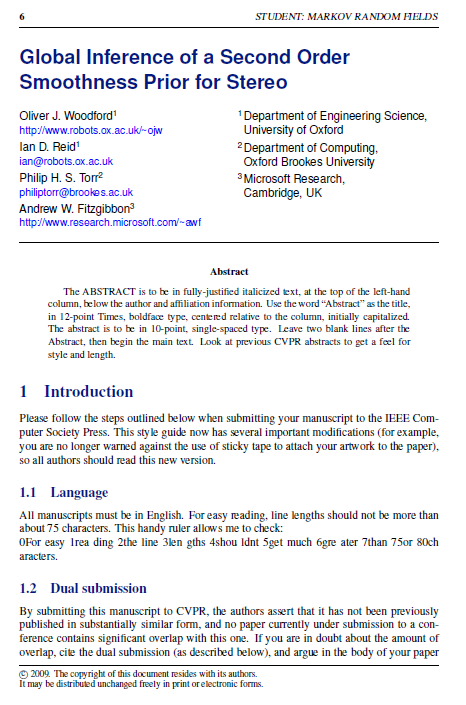
\includegraphics[width=2.8cm]{images/eg1_largeprint.png}}}&
%\bmvaHangBox{\fbox{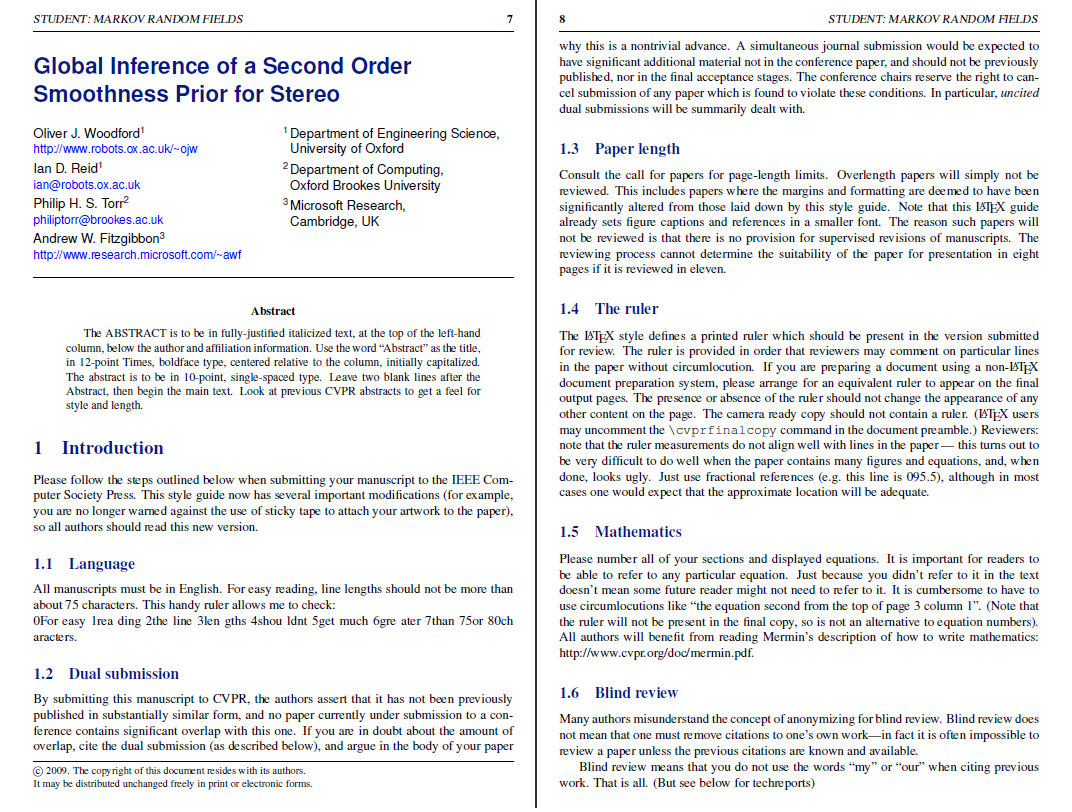
\includegraphics[width=5.6cm]{images/eg1_2up.png}}}\\
%(a)&(b)&(c)
%\end{tabular}
%\caption{It is often a good idea for the first figure to attempt to
%encapsulate the article, complementing the abstract.  This figure illustrates
%the various print and on-screen layouts for which this paper format has
%been optimized: (a) traditional BMVC print format; (b) on-screen
%single-column format, or large-print paper; (c) full-screen two column, or
%2-up printing. }
%\label{fig:teaser}
%\end{figure}

\section{Related Work}

Object detection and pose estimation from conic features is widely studied in 3D vision literature  \cite{dhome_spatial_1990}\cite{safaee-rad_three-dimensional_1992} \cite{werghi_pose_1996} \cite{quan_invariant_1995}. Circular shape is also a popular choice for designing artificial fiducial. Detection of contour points from image and fitting ellipse is a well studied topic \cite{fitzgibbon_direct_1999}. 
%Detection of conic sections from the image is easy and also a widely studied subject [conic fitting, gibbon].
Quan \cite{quan_conic_1996} proposed a two view approach for finding correspondence and 3D reconstruction with conic section. Authors have proposed methods to compute invariants for coplanar conics \cite{forsyth_91} \cite{Ferri_1993}.  
%Various tracking and camera calibration methods use a pair coplanar circular features to compute invariant descriptors. 
A 3D problem is simplified to 2D when coplanar features are recovered and used for correspondence.  
Ying \etal \cite{ying_camera_2007} use a coplanar pair for camera calibration. 
Uchimaya \etal \cite{uchiyama_random_2011} developed invariant descriptors from multiple coplanar circles, and extended the work for deformable model \cite{uchiyama_deformable_2011}.
Work of \cite{lo_pez_de_ipin_a_trip:_2002} \cite{naimark_circular_2002} \cite{pagani_circular_2011} propose a circular marker for 6D pose estimation, no invariants are computed as correspondence is solved by using unique coded pattern around the circle. 
\cite{lo_pez_de_ipin_a_trip:_2002}\cite{pagani_circular_2011} use circular shape to define circle plane in 3D, Additionally use a coded pattern is used encode 6D pose without ambiguity.(Fig). 
Luhmann \cite{luhmann_close_2006} provides detailed account of methods using point circular fiducials in close range Photogrammetry. The current state of the art methods coded patterns are introduced to simplify correspondence problem.
[GOM][AICON] are one of the industrial supplies for close range photogrammetry measurement equipments. 

[Refer Thesis: Comment on catalogue based methods, ]
\paragraph{}
Literature study suggests that, existing methods either provide a solution for coplanar circular features or non-coplanar  coded circular features. The novelty of our method is that it addresses 2D-3D matching problem for non planar circles present in the scene. 


\section{New introduction}

\par 
\parmessage{what is correspondence matching
\begin{itemize}
\item correspondence matching is ...
\item 2 solutions.
\end{itemize}
}
Correspondence matching aims to find correspondences between images or ones between object model and its image projection, thus is one of the key problems in computer vision.
Since perspective transformation differs appearance of a single object on images, correspondence matching needs feature descriptors, which can compute invariant quantities against some transformation, and establishes correspondence by matching the invariant quantities obtained by the descriptors.

%\par 
%\parmessage{projective invariants on primitive features}
%Popular approach to achieve this is to compute projective invariant quantities from primitive features such as points, lines, and conics~\cite{hartley_multiple_2003} and use these invariant quantities for matching.
%Such primitive features are easier to detect from images, therefore invariants on the primitive features have been extensively studied in vision community.
%There exist several works that covered a detailed study on projective invariants and their stability under projective transformation \cite{forsyth_91,gros_projective_1992}
%\yuji{ask Hemal whether the followings are right or not.}
%Quan used \textbf{WHAT} invariant quantity from conic section for finding correspondence between two images and 3D reconstruction \cite{quan_conic_1996}.
%Coplanar conics was used to compute \textbf{WHAT} invariant quantity~\cite{forsyth_91,Ferri_1993} \yuji{is it better to move this invariant quantity on coplanar conics to the next paragraph?}.
%\yuji{any more projective invariants on primitive features?}
%\yuji{will mention why these invariants have used less in this decade.}
%
\par 
\parmessage{Projective invariants on planar objects or primitive features}
\yuji{ask Hemal whether this paragraph is right or not.}
One of the popular approaches use invariant quantities on planar object against perspective transformation.
This type of approaches are based on invariants theory, which has been well-studied in 90s.
There exist several works that covered a detailed study on projective invariants and their stability under projective transformation \cite{forsyth_91,gros_projective_1992}
The invariants theory revealed that primitive features such as points, lines, and conics have invariant quantities against perspective transformation~\cite{hartley_multiple_2003} and the idea is to use these invariant quantities for matching.
Especially, planar projective descriptors, which compute invariant quantities against perspective transformation from planar object, have been investigated.
Quan used \textbf{WHAT} invariant quantity from conic section for finding correspondence between two images and 3D reconstruction \cite{quan_conic_1996}.
Coplanar conics was used to compute \textbf{WHAT} invariant quantity~\cite{forsyth_91,Ferri_1993}.
\yuji{any more projective invariants on primitive features?}
\yuji{will mention why these invariants have used less in this decade.}
\yuji{is here the best place to mention triangulation based matching such as ART?}

\par 
\parmessage{some invariants on fiducial markers}
%\begin{itemize}
%\item use 
%\begin{itemize}
%\item encoded binary pattern (fiducial markers)
%\item some invariants on plane~\cite{Matsunaga2000,uchiyama_random_2011}
%\end{itemize}
%\item can construct a 3D marker by concatenating multiple planar markers
%\end{itemize}
Another approach also using primitive features embeds binary patterns into a planar object, called fiducial markers.
%This type of markers can be made with consumer printers, therefore it is preferred by users making light weight system.
The embedded patterns are extracted from images by adaptive thresholding for matching the correspondence between the marker model and its image projection and then the extracted patterns are decoded for identifying the extracted marker.
The original work by Kato and Billinghurst~\cite{Kato1999} uses the contour of a rectangle but does not use any invariant quantity.
Matsunaga \etal made a special chessboard with different pattern sizes and use cross ratio, which is a projective invariant quantity, defined by intersection of the patterns~\cite{Matsunaga2000}.
Recent works compute perspective~\cite{Nakai2005}, affine~\cite{Nakai2006}, rotation invariants~\cite{Uchiyama2011a} on key-points distribution defined by a set of key-points' location.
\yuji{any disadvantage?}

\par 
\parmessage{local texture descriptors}
%\begin{itemize}
%\item encodes local texture in image
%\item like SIFT
%\item for mobile applications
%\item up to rotation, affine invariants
%\item more idea~\cite{Kurz2012,Lepetit2006}, to handle perspective transformation
%\end{itemize}
Recent trend computes some invariant quantities defined by local texture in image such as SIFT descriptor~\cite{Lowe1999}.
Contrast to the above approaches, this type of approaches does not assume any primitive features in target scene.
Alternatively, the approaches assume textured scene so that we can use the approaches for mobile applications, in which primitive shapes cannot be assumed.
The approaches focus on improving their invariance as well as efficient memory usage so that the matching can run even on powerless processors in mobile phones~\cite{Ke2004,Calonder2010}.
One of the disadvantages of these approaches is that their invariance are up to 2D transformation such as affine and rotation transformation.
To handle view change caused by perspective transformation, we must explicitly learn how invariant quantities are affected by perspective transformation~\cite{Kurz2012,Lepetit2006}

\subsection{Conic invariants under perspective transformation}
\parmessage{conic invariants under perspective transformation}
\yuji{will add more stuff later.}\\
3D objects are known to retain Euclidean invariants rather than projective invariants~\cite{forsyth_91}.
In case of 3D objects, Euclidean invariants are difficult to extract from images due to perspective projection.
Circles have a special property to retain depth information even under projective transformation.
A circle in the 3D world coordinate always appears as an elliptical curve on the image plane.
When the size of circle is known, orientation of circle plane can be defined in 3D (camera coordinates) with a two fold ambiguity~\cite{forsyth_91,safaee-rad_three-dimensional_1992}.
Further, Forsyth \etal~\cite{forsyth_91} proposed that up to three projective invariant can be computed from a pair of non-coplanar circles.
Is is explained that angle between circle planes (angle between surface normals) and distance between centre of the circles are perspective invariant quantities.
Although those invariants were theoretically validated even in early 90s, its practical application have not been explored.

\subsection{Our contribution}
\parmessage{Our contribution}
\yuji{will touch later}\\
%\begin{itemize}
%\item conic pair descriptor
%	\begin{itemize}
%	\item 3D information
%	\item based on invariants of a pair of non-coplanar conics
%	\end{itemize}
%\end{itemize}
\comments{h: our work based on conic invariants}
We propose using these invariants to solve correspondence problem when multiple 3D circular features exist on a model. 
%We \revise{propose}{derive \textit{Conic pair descriptor}} using these invariants \revise{}{computed from a pair of non-coplanar circles} to solve correspondence problem\revise{ when multiple 3D circular features exist on a model}{}. 
In this approach we bring problem from 2D to 3D by computing 3D invariants from image features, then solve 3D-3D matching problem with model.
We introduce $ Conic Pair Descriptor $, which encapsulate invariants computed from elliptical image features to solve the conic ambiguity and provide accurate matching with 3D features.%\revise{In this approach we bring problem from 2D to 3D by computing 3D invariants from image features, then solve 3D-3D matching problem with model.
%We introduce $ Conic Pair Descriptor $, which encapsulate invariants computed from elliptical image features to solve the conic ambiguity and provide accurate matching with 3D features.}
%{With the proposed descriptor, we can extract 3D information from a set of non-coplanar circles, therefore the 2D-3D matching problem is solved as a 3D-3D matching problem.}
The proposed method is first attempt to use these invariants, therefore we also carried out simulations to show stability of invariants against change of perspective.  

\comments{i: our contribution}
%We demonstrate  practical scenario where such method can be used effectively.
Our contribution is a new method to accurately identify image correspondences when multiple identical 3D circular features exist in the scene. We assume that calibration of camera is known and 3D information of features is available. 
Often in Industry based model tracking applications 3D-CAD data is known. Our matching method is suitable for tracking any 3D objects having known circles on different planes. In close range photogrammetry multiple circular markers (Figure. \ref{fig:introProblem}) are placed on 3D models for surface measurements \cite{luhmann_close_2006}. 
These measurements include computation of surface normal and 3D position of each marker. 
This process involves taking multiple images of the model with additional presence of encoded markers in the scene to solve correspondence. 
Once 3D measurements are done our method can be extremely useful to support tracking application without using coded patterns. Similarly various industrial parts having natural circles can be identified and tracked with this method. 
We prepared two car models with circular markers for evaluating our matching method. The proposed method can find corresponding circular marker from a single image, with high accuracy. We also show that our method is stable against false positives detected from the scene. Our method is fast enough to support real-time tracking applications. 



\section{Method}
We will assume that both the 2D and 3D data are already available and focus on the matching method in detail. 
The 3D data includes the surface normal $N_i$, centre position $M_i$ and size $R_i$ (diameter) of the circles present on the model. 
The 2D data includes centre points $m_i$ and conic matrices $C_i$ recovered from the undistorted image. The camera intrinsics ($K$) and distortion parameters are known. 
We have followed the approach presented by Naimark \cite{naimark_circular_2002} for ellipse detection and Farin \etal \cite{farin_geometry_1998} for computation of conic matrices from ellipse parameters. 
%and Fitzgibbon \cite{fitzgibbon_direct_1999} and fitting.

\subsection{Conic Invariants : Theory and Computation}
\label{subSec:ConicInv}
In this part we will explain the theory and computational aspects behind generating Euclidean invariants from the image conics. 
Let the camera projection centre be assumed as the vertex of a cone having the world circle is as its base.
Now the image plane can be considered as a cutting plane $\pi$, which always creates an elliptical cross section of the cone.  
A rotation transformation $R_c$ can be applied to the camera coordinate system such that the new image plane $\pi'$ intersects the cone as a perfect circle, with the z-axis passing through the centre of both the circles. 
The normal of the plane ($\pi'$) is same as the base of the cone, therefore a normal $Nc_i$ to the plane $ \pi $ can be computed using $R_c$. 
Similarly, using $ R_i $, distance between the plane $ \pi' $ and the base of the cone can be computed. 
Additionally, 3D position of circle centre $Mc_i$ can be computed in the original camera coordinate frame.
The normal $Nc_i$ and the point $Mc_i$ are sufficient to define the orientation of the circle in camera coordinate system.
$ R_c $ is a combination of two rotations, one of the two has $\pm \phi$ rotation ambiguity, which in turn introduces a two fold ambiguity in the solution (See Eq.\ref{Eq:Backprojection}). We will refer the ambiguity as \textit{Conic ambiguity} and the method to obtain plane orientation as \textit{Ellipse backprojection}. The mathematical model for \textit{Ellipse backprojection} is extensively covered by both Forsyth \etal \cite{forsyth_91} and Diego \cite{lo_pez_de_ipin_a_trip:_2002}. 
\begin{align} \label{Eq:Backprojection}
\text{Ellipse Backprojection}(m_i,C_i) &\rightarrow \pi({Nc_i}^1,{Mc_i}^1),\pi'({Nc_i}^2,{Mc_i}^2) \\ \nonumber
\text{Ellipse Backprojection}(m_j,C_j) &\rightarrow \pi({Nc_j}^1,{Mc_j}^1),\pi'({Nc_j}^2,{Mc_j}^2)
\end{align}
Forsyth \etal \cite{forsyth_91} explained that in case of three dimensional objects invariant descriptors consists of Euclidean invariants rather than projective invariants. 
Various invariants can be computed from a pair of non-coplanar circles based on Ellipse backprojection. 
We use following invariants for our method, 
\begin{itemize}
	\item \textbf{Angle between planes} ($\theta$) : It is same as the angle between the surface normals 
	(i.e. $ \angle(Nc_i,Nc_j) $). $\theta$ can be recovered from the image conics without knowledge of the circle size , however due to \textit{Conic ambiguity} $ \theta $ will have 4 solutions out of which only one is correct. 
	\item \textbf{Distance between circle centres} : This is the distance between $ Mc_i$ and $ Mc_j $. The length of the vector $d_c$ is invariant (object scale should be known) and consistent despite of the ambiguity. 
\end{itemize}
%It should be noted that ambiguity of Ellipse Backprojection produces 4 solutions for $\theta$, only one of which is correct. 
%Other invariants can be computed from recovered normal and centre values. These invariants are unstable \cite{forsyth_91} as the error from both recovered components influences the computation.
The quality of recovered plane from \textit{Ellipse backprojection} depends on distance from the camera $ r $ and the viewing angle $ \eta $(angle between the image plane and the circle plane)\cite{werghi_pose_1996}. 
We performed simulations to understand behaviour of Ellipse Backprojection with respect to both $ r $ and $ \eta $. The parameter $ r $ is varied from 0.5 to 2 m and $ \eta $ from 0-70$^\circ$ in step wise manner, while recording 100 iterations at each step (Fig. \ref{fig:InvariantRecovery}). Realistic values have been assumed for camera intrinsics and size of circle ($ R_i $ = 5,8,12 mm).
Figure. \ref{fig:InvariantRecovery} shows results recorded with $ R_i = 12 $, and image noise as $ \sigma = 0.3 $. 
The results suggest, at low viewing angles 0-10$^\circ$ both normal and centre estimation errors are high, at any given distance. 
This can be explained by the fact that for lower values of $ \eta $ image projection of a circle is circular and not elliptical, therefore recovery of elliptical parameters may have errors. 
We also observe that the estimation error grows with camera distance, however the error in normal recovery appears less sensitive to camera distance than the error in centre recovery. 
The results obtained with $ R_i = 5,8~ mm $ show similar pattern, however the magnitude of error is higher as the image projection become smaller in the image. 
We also computed and compared the results of estimated centres $ {Mc_i}^1 $ and $ {Mc_i}^2 $. The maximum distance recored between the two is $ \leq $  0.1 mm for $R_i$ = 12 mm, this suggests that ambiguity can be neglected for the recovered centre position. The centre recovery is prone to higher errors with higher camera distances, however it produces a consistent solution for invariant $ d_c $. After performing \textit{Ellipse backprojection} we have essentially transformed our problem from image space to three dimensional space. 

\begin{figure}
\centering
\begin{tabular}{cc}
\bmvaHangBox{\fbox{\includegraphics[width=4cm,keepaspectratio=true]{images/centerEstimationErrorR6_N3.png}} }&
\bmvaHangBox{\fbox{\includegraphics[width=4cm,keepaspectratio=true]{images/NormalRecoveryError_R6_3.png}} } \\
%\caption{\label{fig:matchingProblem}}
%\caption{\label{fig:matchingProcess}}
(a)&(b)
\end{tabular}
\caption{ Ellipse backprojection results at different camera distance and viewing angles,Image noise = $ \sigma = 0.3 $,$ \phi = 12 mm $ ;
(a) Error in Centre ($ Mc_i $) (b) Error in Normal ($ Nc_i $) \label{fig:InvariantRecovery} }
\end{figure}

\subsection{Descriptor Generation}
This part mainly discusses generation of \textit{Conic pair descriptor} from Euclidean invariants. 
The invariants for 3-D model are computed from available 3D data ($M_i,N_i$) without any ambiguity (See Eq. \ref{Eq:3Ddescriptors}). 
The same set of invariants can be computed from corresponding image features, where the recovered $ d_c $ component is unique and $ \theta $ component has 4 solutions (See Eq. \ref{Eq:2Ddescriptors}). 
In our approach we pursue the idea that the existence of multiple features on the model can be used to overcome the Conic ambiguity problem. 
The principle idea is to generate descriptors from conic invariants to perform a descriptor matching to obtain $ m_i \leftrightarrow M_i $ correspondence.
The proposed \textit{Conic pair descriptor} structure,
%which also encapsulates the conic ambiguity, 
\begin{align}
\textit{Conic pair descriptor}_{model} &= V_{p} \langle d_c,\theta \rangle_{i,j} \label{Eq:3Ddescriptors} \\
\textit{Conic pair descriptor}_{image} &= v_{q} \langle  d_c,\theta_{11},\theta_{12},\theta_{21},\theta_{22} \rangle_{i,j} \label{Eq:2Ddescriptors} 
\end{align}
where $V_{p}$ represents world circles $i,j$ and $v_{q}$ represents image conic pair $i,j$. 
The reader should note that given a set of points and their corresponding normals in 3D camera space, PFH descriptor \cite{RusuDoctoralDissertation} also computes similar invariants. In this case, the concept can not be applied to the results of \textit{Ellipse backprojection} as the \textit{Conic ambiguity} restricts us from computing a unique set of invariants. 
Unlike popular methods, a \textit{Conic pair descriptor} represents two features at same time. 
In order to uniquely represent a single conic using Euclidean invariants, at least more than two conic features are required. 
Addition of each conic feature adds 3 wrong solutions of $ \theta $ in the descriptor, additionally the matching must rely on detection of all the conics used for descriptor computation. 
We propose matching $ v \leftrightarrow V $ first, thereby finding a corresponding conic pair, further we solve individual correspondence $ m_i \leftrightarrow M_i $ problem. 
Descriptor $ v_{\{1..q\}} $ are computed among each pair of detected $ n $ image conics, where $ q = \binom{n}{2} $. 
$ V_{\{1...p\}} $ are computed off-line as the 3D data is already available. In this case for $ l $ world circles  $ p \leq \binom{l}{2} $, as pairs not likely to appear in same image can be rejected. 
After computing the \textit{Conic pair descriptors} the following 3 step matching approach is used to achieve $ m_i \leftrightarrow M_i $ correspondences. 

% -> Figure explaining the issue
%\begin{figure}[!ht]
%\centering
%\subfloat[A problem showing four image points, and their correspondence with world points (1-A,2-B,C-3) and one false positive (D)\label{fig:matchingProblem} ]
%{\includegraphics[width = 0.45\textwidth ]{images/matchingProblem.png} }
%\subfloat[Image shows the simplified matching process for the problem suggested in (a), partial results of all 3 steps are shown. \label{fig:matchingProcess}  ]
%{\includegraphics[width = 0.45\textwidth]{images/matchingProcess.png} }
%\caption{Matching problem and the overview of the method to generate correspondence hypothesis :\label{fig:matchingAndProblem}}
%\end{figure}

\begin{figure}
\centering
\begin{tabular}{cc}
\bmvaHangBox{\fbox{\includegraphics[width=4cm,keepaspectratio=true]{images/matchingProblem.png}} }&
\bmvaHangBox{\fbox{\includegraphics[width=4cm,keepaspectratio=true]{images/matchingProcess.png}} } \\
(a)&(b)
\end{tabular}
\caption{ Matching problem and the overview of the method to generate correspondence hypothesis ;
(a) A problem showing four image points, and their correspondence with world points (1-A,2-B,C-3) and one false positive (D) (b) Image shows the simplified matching process for the problem suggested in (a), partial results of all 3 steps are shown. \label{fig:matchingAndProblem}}
\end{figure}

\subsection{Step 1: Pairwise Initial Matching}
\label{subSec:PIM}
In the first stage of the matching process we compare the \textit{Conic pair descriptors}.
% ($ V \leftrightarrow v $).
The objective is to reduce complexity of the problem by finding the possible pair correspondences ($ v \leftrightarrow V $). 
First the unique component($ d_c $) between the descriptors is compared, if matched then ($ \theta $) component of $ V $ is compared with all 4 values of $ \theta $ component in $ v $ (Ref. Algorithm \ref{algo:PIM}). 
$ T_{d_c} $ and $ T_\theta $ are the threshold values used to compare the respective components. 
The stage may result in \textit{one to many} type of relation between descriptors. This can be either due to similar feature orientation on object or due to presence of the \textit{Conic ambiguity}. 
The reader should note that a descriptor represents a pair of conics, therefore the stage is called pairwise matching.
%Even an accurate match does not solve individual correspondence in this stage. 
The example given in Figure \ref{fig:matchingAndProblem} shows possible outcome of step 1 with respect to the given example problem. 

\begin{algorithm} \label{algo:PIM}
\SetKwData{threeDFv}{$ V_{p} $}\SetKwData{twoDFv}{$ v_{q} $}
\SetKwData{ThresholdD}{$T_{d_c} $}\SetKwData{ThresholdA}{$T_\theta $}
\SetKwFunction{compareDist}{compare$d_c$}\SetKwFunction{compareAngle}{compare$ \theta $}
\SetKwFunction{Save}{SavePairResult}
\emph{Goal : Find all possible \threeDFv similar to \twoDFv} \;
\emph{Initialisation : \ThresholdD = 10 , \ThresholdA = 5} \; 
\ForAll{ 3D Feature Descriptors ($ V $), $ p \leftarrow 0 $ \KwTo $ n $}{	
	\ForAll{ 2D Feature Descriptors ($ v $), $ q \leftarrow 0 $ \KwTo $ l $}{
			% Project conic points 
			\If (\tcp*[h] {compares $ d_c $ component} ){ \compareDist{\threeDFv,\twoDFv} $ < $ \ThresholdD } {
				\If (\tcp*[h] {compares $ \theta $ component} ){ \compareAngle{\threeDFv,\twoDFv} $ < $ \ThresholdA }{
				\tcp{ All 4 solutions of $ \theta $ in $ v_q $ are checked } \;			
				\Save{$ p,q $} \tcp{Save matching descriptor pair} \;
				}
			}
		}	
	}
\caption{Pairwise Initial Matching algorithm}
\end{algorithm}

%------------------------------------------------------------------------- 
\subsection{Step 2: Pointwise Triplet Matching}
In this stage we simplify the problem further and obtain hypothesis on point wise matching ($ m_i \leftrightarrow M_i $) by performing a verification on $ v \leftrightarrow V $ matching results. 
The objective is to compare the results of step 1 to identify and reject false descriptor matches. 
We seek three $ v \leftrightarrow V $ results, such that they complement each other to form a unique three points $ m_i \leftrightarrow M_i $ hypothesis.
A simple two stage approach is proposed to generate a triplet matching hypothesis,
\begin{enumerate}
\item[1] Find any two results of Pairwise Initial Matching in which both the image and the model descriptors represent one and only one common conic. If such results exist then an initial triplet matching hypothesis can be proposed. 
\[
 V_{12} \leftrightarrow v_{AB},V_{13} \leftrightarrow v_{AC } \xrightarrow{\text{Triplet Hypothesis}} [1~2~3] \leftrightarrow [A~B~ C]
\]
In the example above we can see that world conic 1 and image conic A is common among the two solutions. We form a 3 point matching hypothesis with these results. 
\item[2] Find a new descriptor matching pair which can verify the triplet matching hypothesis formed in the previous stage (e.g. $ V_{23} \leftrightarrow v_{BC}$).
\end{enumerate}
The verified triplets are saved and others are rejected. 
The results may also contain false triplet matches (Fig. \ref{fig:matchingAndProblem}). 
If $ x $ number of results are generated in step 1, the number of pairs compared in this stage is $ \binom{x}{3} $. 

\subsection{Step 3: Correspondence Hypothesis }
\label{subSec:CHypo}
In this final step results of triplet matching are combined and a voting matrix is generated (Fig. \ref{fig:matchingAndProblem}). 
A $ m_i \leftrightarrow M_i $ pair having maximum votes in the matrix is proposed as a correspondence hypothesis. 
In case of conflicting votes the respective $ m_i \leftrightarrow M_i $ relation is not considered. 
A minimum of 3 correspondence are required to compute the pose of the object \cite{lepetit_monocular_2005}, if camera intrinsics are known. 
A pose of the object can be computed by selecting top 3 correspondence results and verify other correspondences obtained from the matrix. 
If only 3 out of $ n $ conics are detected in the image, verification with pose is not possible and results may not be reliable. 

\section{Evaluation}
In this section we will cover experiments carried out to comment on accuracy and robustness of the algorithm. 
%To the best of our knowledge no other application has attempted using the euclidean invariants generated by circles. 
The reader should note that the problem of achieving single image 2D-3D correspondences for non-coplanar circles has not been addressed earlier. 
Therefore, alternative methods for comparison are not available. 
We prepared test models by attaching circular markers of size $ \phi $ = 12 mm ($ M_i = 20 $) and 5mm ($ M_i  = 26$). The markers used are widely accepted and used in the Industrial domain for Photogrammetric measurements.     
3D measurements for the markers are done with state of the art metrology system, and the ground truth is established by giving each model point a unique ID in the database. 
The markers are attached randomly and coplanar placement is avoided. 
A high resolution (2560x1920) camera is used for the experiments and MATLAB is used for synthetic experiments. 

\subsection{Experiment 1 : Descriptor Matching vs Marker Orientation}
This experiment is carried out synthetically to observe the effect of orientation of the circles on the descriptor matching results.
Two circle planes are placed in different orientations and images are captured (noise $ \sigma = 0.3 $) from 1000 different camera positions for each orientation. 
The control parameters, the distance between circle centres $ d_c $ is varied from 10 - 150 (mm) and the angle between the planes $ \theta $ is varied from 10 - 80$ ^\circ $. 
The objective is to recover the descriptor components $ d_c $ and $ \theta $ from the images, compare them with ground truth and measure the success rate. 
Realistic values are used for camera intrinsics, $ T_{d_c} $ = 10 and $ T_\theta $ = 5 are kept constant. 
%Camera rotation parameters is set -70 to 70 and translation parameters for 
Camera positions are chosen at random from a defined range, range for x-y-z rotation is -70 to 70, x-y translation range is -500 to 500 mm, z-translation (Camera distance) range is 500-2000 mm. 

\begin{table}
\centering
\caption{Descriptor Matching Analysis } \label{table:MatchingSuccess}
\begin{tabular}{|c | c | c | c | c |}
\hline
$ R_i $ & $ \theta $ & $ d_c $ & Camera Distance (mm) & Min-Max Success($ \% $) \\ \hline
5 & 10-40 & 10-150 & 500-2000 & 58-82 \\
 & 40-80 & 10-150 & 500-2000 & 35-65 \\ \hline
% & 0-40 & 1200-2000 & 55-80 \\
% & 40-90 & 1200-2000 & 35-55\\ 
12 & 10-40 & 10-150 & 500-2000 & 64-86 \\
& 40-80 & 10-150& 500-2000 & 40-69 \\ \hline
%& 0-40 & 10-150& 2000-4000 & 40-60 \\
%& 40-90 & 10-150 & 2000-4000 & 20-40 \\ \hline
 20 & 10-40 & 10-150 & 500-2000 & 74-92 \\
 20 & 40-80 & 10-150 & 500-2000  & 48-77 \\ \hline 
\end{tabular} \\
\label{tab:Exp1}
\end{table}
The table \ref{table:MatchingSuccess} provides summary of key observations made during the experiment. 
The matching success shows inversely proportional relation with $ \theta $, independent of $ d_c $. 
We learn that descriptor matching is influenced more by angle between planes than distance between the circle centres. 
It is also seen that success of matching can be improved by increasing the size of the circles. 
%even at higher values of $ \theta $. 
This experiments suggest that when features placement is possible, it is advised to choose larger circles or surfaces with lower plane angles for improved matching results. 

%------------------------------------------------------------------------- 
\subsection{Experiment 2 : Correspondence Matching vs Threshold Settings}
In case of model with natural features choice over size or placement is not available.
The aim of this experiment is to understand the role of threshold values $ T_{d_c}$ and $ T_\theta $ in $ m_i \leftrightarrow M_i $ matching results. 
In order to perform this experiment we took 75 images of car model with 12 mm markers (Distance Range 500-2000 mm). 
%All the results (Table.~\ref{tab:Exp2}) are verified with ground truth data manually. 
As suggested in Sec. \ref{subSec:CHypo}, each image has at least 4 detected conics. 
The results are considered \textit{Not Converged} (NC) in case of less than 3 $ m_i \leftrightarrow M_i $ results.
%If hypothesis proposes less than 3 $ m_i \leftrightarrow M_i $ results we consider it as \textit{Not Converged}. %\textit{Correct} results are divided in two categories purely to provide detailed overview of algorithm performance. \textit{ Complete} refers to $ m_i \leftrightarrow M_i $ hypothesis being 100\% correct, \textit{Partial} results suggest that some of the matching results (excluding top 3 voted pairs) are not correct.  

%\begin{table}
%\centering
%\caption{Correspondence matching with varying threshold settings } \label{table:ThresholdEffect}
%\begin{tabular}{ | c | c | c | c | c | c |}
%\hline
%\multicolumn{2}{|c|}{Settings} & NC & \multicolumn{2}{|c|}{Correct} & Wrong \\ \hline
%$ T_\theta $ & $ T_{d_c} $ & {} & Complete & Partial & {}\\ \hline
%5 & 5  & 13 & 62 & 0 & 0 \\
%5 & 10 & 8 & 67 & 0 & 0 \\
%5 & 15 & 4 & 67 & 0 & 4 \\ \hline
%3 & 5  & 28 & 47 & 0 & 0 \\
%3 & 10 & 21 & 50 & 4 & 0 \\
%3 & 15 & 19 & 52 & 1 & 3 \\ \hline
%\end{tabular} \\
%\label{tab:Exp2}
%\end{table}

\begin{table}
\centering
\caption{Correspondence matching with varying threshold settings } \label{table:ThresholdEffect}
\begin{tabular}{ | c | c | c | c | c | c| c |}
\hline
$ T_\theta $ & $ T_{d_c} $ & NC & Positive & FP & Precision & Recall \\ \hline
%$ T_\theta $ & $ T_{d_c} $ & {} & Complete & Partial & {}\\ \hline
5 & 5  & 13 & 62 & 0 & 100 & 82.6 \\
5 & 10 & 8 & 67 & 0 & 100 & 89.33\\
5 & 15 & 4 & 67  & 4 & 94.36 & 89.33\\ \hline
3 & 5  & 28 & 47  & 0 & 100 & 62.66 \\
3 & 10 & 21 & 54  & 0 & 100 & 72 \\
3 & 15 & 19 & 53  & 3 & 94.64 & 70.66 \\ \hline
\end{tabular} \\
\label{tab:Exp2}
\end{table}

In Sec. \ref{subSec:ConicInv}, we learned that $ d_c $ recovery is weak and therefore a flexible threshold may be appropriate for matching. 
The results ( Table. \ref{tab:Exp2}) show that higher flexibility in $ T_{d_c} $ impacts both precision and recall values in negative manner. 
On the other hand, very stringent thresholds lead to lower recall values. Therefore, a right balance of threshold can be selected to achieve higher precision and recall rates. Our preferred settings for experiments is $ T_{d_c} = 10 $ and $ T_\theta = 5 $. The selection may require change based on density of the features. 

\subsection{Robustness against false positives}


%------------------------------------------------------------------------
\subsection{Time Analysis}
In this experiment we focus on analysing time consumed by the matching method when introduced into a tracking application. 
Two cameras CAM 1 (2560 x 1920) and CAM 2 (640x480) are used for tracking, the results presented are averaged over 100 frames. 
The results show that our method takes $ \leq 1\% $ time from in the tracking pipeline. In terms of frame rates we achieve 2-3 FPS with CAM 1 and 7-8 FPS with CAM 2. Additionally, an exhaustive experiment with 90-140 false positives in the scene shows that matching consumes maximum time in the pipeline (0.7 FPS). Limited tracking range ($<$ 500 mm) of CAM 2 does not allow experiment with such large number of false positives. 
\begin{table}
\caption{Time Analysis}\label{table:trackPerformance}
\centering
\begin{tabular}{|c | c | c | c |}
\hline 
Algorithm Stage & \multicolumn{2}{|c|}{CAM 1} & CAM 2\\ \hline
{} & Model & Model + FP & Model \\ \hline 
Image Undistortion & 39.53\% & 12 & 11.79 \\
Marker Detection & 38.51 & 34 & 30.75 \\
Correspondence Matching & 0.35 & 44.2 & 1.34 \\
%Descriptor Generation & 0.10 & 0.33 \\
%Descriptor Matching & 0.25 & 1.01 \\
Pose Estimation & 21.61 & 9.8 & 56.12 \\ \hline
\end{tabular}
\end{table}

\section{Conclusion \& Future work }
%----------- Do I mention conic ambiguity? 
In this paper we have demonstrated a successful approach for solving 2D-3D correspondence matching problem for non-coplanar circular features from a single image. 
We propose a new \textit{Conic descriptor} which represents euclidean invariants generated by a pair of non-coplanar circles.
Our method can successfully define correspondences for more than 3 circular features are present in the scene. 
The proposed method is the first to address the correspondence matching using these invariants since its introduction in the 90s.
Our contribution also includes providing detailed understanding of behaviour of invariants with respect to orientation and size of the circles. The major factors affecting matching are also discussed to optimize the method for best possible matching results based on application (threshold settings, circle size, camera distance). 
The results of the experiments support our claim, that the method is fast, reliable and robust against false positives.
Our method can be used for object tracking or object identification in Industrial scenario, where natural or artificial circular features exist on the models. However, the method is generic and can be used for any application dealing with non coplanar circles. 
The 3D information of the features on the model and camera calibration are the only prerequisites for matching. 
The reader should also note that algorithm may not perform well with symmetric or coplanar arrangement of circular features. 

In context of future work, we would like to improve the method to be able to handle features of different sizes simultaneously.
Also a faster matching strategy is required to handle large number of feature points and false positives. We would like to use the same invariants to compute 2D-2D correspondence matching between two images in order to generate the 3D data which is a prerequisite now. We also consider using such matching algorithm to support creating 3D markers for monocular Augmented Reality applications. This can be a cheap alternative to conventionally used 3D spherical markers.  


\bibliography{egbib}
\end{document}
